\documentclass[class=report, crop=false, 12pt,a4paper]{standalone}
\usepackage{enumitem}
\usepackage{multicol}
\usepackage{graphicx}
\usepackage{float}
\usepackage{amsmath}
\usepackage{amssymb}
\usepackage{mathtools}
\usepackage{siunitx}
\usepackage{commath}
\usepackage{array}
\usepackage{natbib}
\usepackage{tikz}
\usepackage{cancel}
\usepackage[a4paper,width=150mm,top=25mm,bottom=25mm]{geometry}
\allowdisplaybreaks
\setlength{\parindent}{0pt}
\numberwithin{equation}{section}
\begin{document}
\begin{center}
  09/02/2021
\end{center}
\subsection*{Importance of Combustion}
\begin{figure}[H]
  \centering
  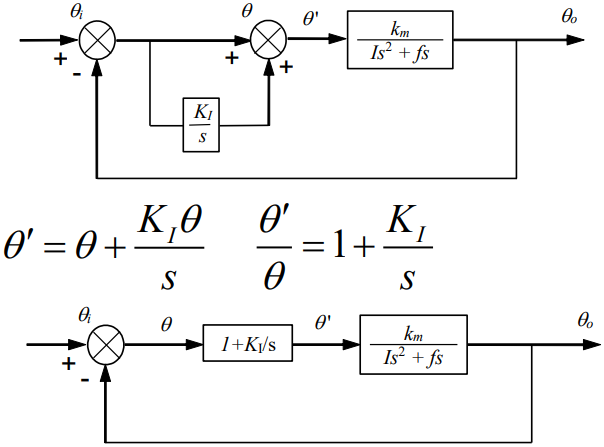
\includegraphics[width = 0.9 \textwidth]{../img/diagram127.png}
  \caption{}
\end{figure}
Combustion is predominant source of useful energy, and predominant source of pollutant and CO$_2$ emissions.
\subsection*{What Is Combustion?}
Chemical Reaction:
\begin{itemize}[noitemsep]
  \item Bonds within the molecules of the reactants are broken.
  \item Atoms and electrons are rearranged to \textbf{form new chemical species} called products.
\end{itemize}
Combustion:
\begin{itemize}[noitemsep]
  \item Rapid oxidation of fuel for heat release:
\end{itemize}
\begin{gather}
  \text{Fuel} + \text{Oxidizer} \longrightarrow \text{Products} + \textbf{Heat Release}
\end{gather}
\section{Global and Elementary Reactions}
\subsection{Study of Chemical Reactions}
\subsubsection{Overall/Global Reaction}
Statement of mass and number of atoms conservation.
\begin{gather}
  2H_2 + O_2 \longrightarrow 2H_2O
\end{gather}
\subsubsection{Elementary Reaction}
Direct results of collisions between reactant molecules. Combustion usually consists of a large set of elementary reactions, e.g. hydrogen combustion:
\begin{gather}
  H + O_2 \longleftrightarrow OH + O \\[5pt]
  O + H_2 \longleftrightarrow OH + H \\[5pt]
  H + OH + R \longleftrightarrow H_2O + R \\[5pt]
  H + O + R \longleftrightarrow OH + R
\end{gather}
Chemical Kinetics: Study of mechanisms and rates of chemical change.
\subsection{Chemical Complexity}
\textbf{Reality:} Detailed chemical mechanisms involve a huge number of elementary reactions and intermediate species.
\begin{figure}[H]
  \centering
  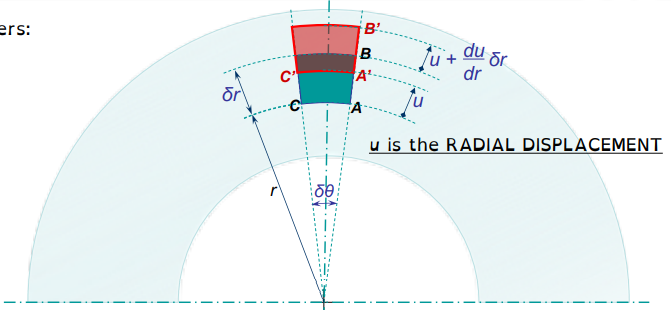
\includegraphics[width = 0.7 \textwidth]{../img/diagram128.png}
  \caption{}
\end{figure}
\subsection{Fuel and Oxidizer}
Fuel:
\begin{itemize}[noitemsep]
  \item Liquids: e.g. gasoline, diesel, kerosene;
  \item Gases: e.g. natural gas;
  \item Solids: e.g. coal.
  \item Most common fuels : \textbf{Hydrocarbons} ($\mathbf{C_xH_y}$), e.g., Methane ($CH_4$), propane ($C_3H_8$), octane ($C_8H_{18}$), gasoline (average $C_{7.2}H_{12.6}$), diesel (average $C_{12}H_{23}$)
  \item Bio-fuels : \textbf{Usually} ($\mathbf{C_xH_yO_z}$), e.g., Methanol ($CH_3OH$), ethanol ($C_2H_5OH$)
\end{itemize}
Oxidizer:
\begin{itemize}[noitemsep]
  \item In most combustion applications, air provides the needed oxygen;
  \item However, pure oxygen ($O_2$) can be used, called oxy-fuel combustion, for carbon capture and storage
\end{itemize}
\subsection{Fuel Composition}
\begin{figure}[H]
  \centering
  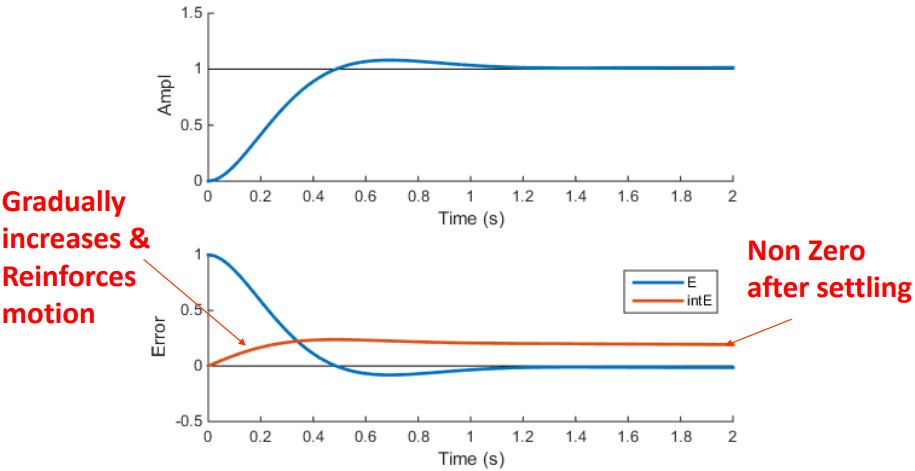
\includegraphics[width = 0.65 \textwidth]{../img/diagram129.png}
  \caption{}
\end{figure}
\section{Combustion in Air}
\subsubsection{Combustion in Dry Air:}
\begin{align*}
  \text{Fuel (F)} + &\text{Dry Air (A)} \longrightarrow \text{Carbon Dioxide} \ (CO_2) + \text{Water} \ (H_2O) + \text{Nitrogen} \ (N_2) \\[5pt]
  \text{Dry Air (A)} &= 21\% \ \text{by volume of Oxygen} \ (O_2) + 79\% \ \text{by volume of Nitrogen} \ (N_2) \\[5pt]
  &= 1 \ \text{unit volume of Oxygen} \ (O_2) + 3.76 \ \text{unit volume of Nitrogen} \ (N_2)
\end{align*}
\subsubsection{Combustion in Moist Air:}
\begin{gather*}
  \text{Fuel (F)} + \text{Moist Air (A)} \longrightarrow \text{Carbon Dioxide} \ (CO_2) + \text{Water} \ (H_2O) + \text{Nitrogen} \ (N_2) \\[5pt]
  \text{Moist Air (A)} = 1 \ \text{unit mass of Oxygen} \ (O_2) + 3.29 \ \text{unit mass of Nitrogen} \ (N_2) \\ 
  + 4.29\omega \ \text{unit mass of Water Vapour} \ (H_2O)
\end{gather*}
\subsection{Air/Fuel Ratio and Fuel/Air Ratio}
Air/Fuel Ratio by Mass:
\begin{gather}
  AF = \frac{\text{mass of air}\ (m_{air})}{\text{mass of fuel}\ (m_{fuel})} = \frac{x_{air}}{x_{fuel}} = \frac{n_{air}}{n_{fuel}}\frac{M_{air}}{M_{fuel}}
\end{gather}
Fuel/Air Ratio by Mass:
\begin{gather}
  FA = \frac{1}{AF}
\end{gather}
Air/Fuel Ratio by Volume:
\begin{gather}
  \overline{AF} = \frac{\text{volume of air}\ (V_{air})}{\text{volume of fuel}\ (V_{fuel})} = \frac{n_{air}}{n_{fuel}} = \frac{y_{air}}{y_{fuel}}
\end{gather}
Relationship:
\begin{gather}
  AF = \overline{AF}\frac{M_{air}}{M_{fuel}}
\end{gather}
\subsection{Stoichiometric Combustion in Air}
\subsubsection{Stoichiometry:}
Chemically exact proportion of fuel and air for complete burning of fuel.
\subsubsection{Stoichiometric Combustion of Hydrocarbons in Dry Air:}
\begin{gather}
  C_xH_y + a(O_2 + 3.76N_2) \longrightarrow b\ CO_2 + c\ H_2O + 3.76d\ N_2
\end{gather}
Balance of atom number for each element:
\begin{align}
  C: \ \ \ &x = b \\[5pt]
  H: \ \ \ &y = 2c \\[5pt]
  O: \ \ \ &2a = 2b + c \\[5pt]
  N: \ \ \ &2\cdot 3.76a = 2\cdot 3.76d
\end{align}
Therefore, the stoichiometric coefficients:
\begin{align}
  b &= x \\[5pt]
  c &= \frac{y}{2} \\[5pt]
  a &= x + \frac{y}{4} \\[5pt]
  d &= a
\end{align}
The mass balance equation for stoichiometric combustion:
\begin{gather}
  C_xH_y + \left(x+\frac{y}{4}\right)(O_2 + 3.76N_2) \longrightarrow xCO_2 + \frac{y}{2}H_2O + 3.76\left(x+\frac{y}{4}\right)N_2
\end{gather}
Note:
\begin{itemize}[noitemsep]
  \item The mass, atom/mole number of each element are conserved.
  \item The total mass of reactants equals that of the products.
  \item The total mole numbers of reactants and products are not usually the same.
\end{itemize}
\subsubsection{Stoichiometric Combustion of Hydrocarbons in Air:}
\begin{gather}
  C_xH_y + \left(x+\frac{y}{4}\right) \left(O_2 + \frac{0.79}{0.21}N_2\right) \longrightarrow xCO_2 + \frac{y}{2}H_2O + \left(x+\frac{y}{4}\right)\frac{0.79}{0.21}N_2
\end{gather}
Stoichiometric Air/Fuel Ratio (by volume):
\begin{gather}
  \overline{AF}_{stoi} = \left(x+\frac{y}{4}\right)\left(1+\frac{0.79}{0.21}\right)
\end{gather}
Stoichiometric Air/Fuel Ratio (by mass):
\begin{gather}
  AF_{stoi} = \frac{\left(x+\frac{y}{4}\right) \left(32+\frac{0.79}{0.21}\cdot 28\right)}{12x + y}
\end{gather}
For typical petroleum-based fuels, $AF_{stoi} = 14 \sim 15$.
\subsection{Equivalence Ratio}
Equivalence ratio is a measure of the proportion of fuel and air in a reactive mixture relative to its stoichiometric value. \\\\
Equivalence Ratio (by Mass):
\begin{gather}
  \phi = \frac{(FA)_{actual}}{(FA)_{stoi}} = \frac{(AF)_{stoi}}{(AF)_{actual}}
\end{gather}
Equivalence Ratio (by Volume):
\begin{gather}
  \overline{\phi} = \frac{(\overline{FA})_{actual}}{(\overline{FA})_{stoi}} = \frac{(\overline{AF})_{stoi}}{(\overline{AF})_{actual}}
\end{gather}
\begin{align*}
  \phi > 1.0 &\longrightarrow \text{fuel-rich mixture/combustion} \\[5pt]
  \phi = 1.0 &\longrightarrow \text{stoichiometric mixture/combustion} \\[5pt]
  \phi < 1.0 &\longrightarrow \text{fuel-lean mixture/combustion}
\end{align*}
\subsection{Actual Combustion Process}
In an actual process:
\begin{itemize}[noitemsep]
  \item Combustion take places in \textbf{tens or hundreds of elementary reactions}.
  \item Usually a \textbf{huge number of intermediate species} are generated.
  \item A combustion process is almost always \textbf{incomplete}.
  \item In addition to the usual products $CO_2$ and $H_2O$, there are \textbf{harmful emissions} from combustion such as unburned $HC$, $CO$, $NO_x$ and soot.
  \item The combustion process is strongly affected by fluid dynamics (in particular, \textbf{turbulence}) and \textbf{mixing}. 
\end{itemize}
\section{Open System Energy Analysis of Combustion Processes}
\begin{figure}[H]
  \centering
  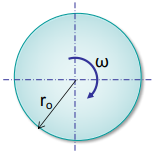
\includegraphics[width = 0.9 \textwidth]{../img/diagram130.png}
  \caption{}
\end{figure}
Assumptions:
\begin{itemize}[noitemsep]
  \item SSSF (steady state simple fluid)
  \item $\Delta KE = \Delta PE = 0$
  \item No mechanical work
\end{itemize}
Steady State Energy Balance:
\begin{gather}
  \cancel{\frac{\dif E_{CV}}{\dif t}} = \dot{Q} + \cancel{\dot{W}} + \sum_{in}\dot{m}_{in}\left(h+\cancel{\frac{v^2}{2}}+\cancel{gz}\right)_{in} - \sum_{out}\dot{m}_{out}\left(h+\cancel{\frac{v^2}{2}}+\cancel{gz}\right)_{out} \\[5pt]
  \dot{Q} = \sum_{out}\dot{m}_{out}h_{out} - \sum_{in}\dot{m}_{in}h_{in}
\end{gather}
Combustion heat release (on a mass basis):
\begin{gather}
  Q = \sum_{P}(m_i h_i) - \sum_{R}(m_i h_i) = H_P - H_R
\end{gather}
Combustion heat release (on a molar basis):
\begin{gather}
  Q = \sum_{P}(n_i \overline{h}_i) - \sum_{R}(n_i \overline{h}_i) = H_P - H_R
\end{gather}
\subsection{Energy Change in a Chemical Reaction}
\begin{figure}[H]
  \centering
  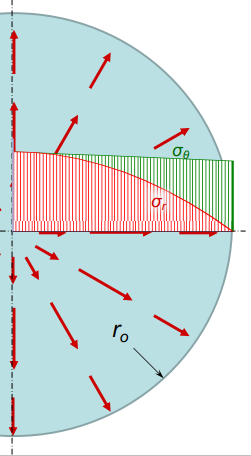
\includegraphics[width = 0.9 \textwidth]{../img/diagram131.png}
  \caption{}
\end{figure}
$\Delta H_r^\circ$ is enthalpy change in combustion at standard reference temperature $T_o$. \\
$\Delta H_r$ is enthalpy change in combustion at an arbitrary temperature $T$.
\section{Enthalpy of Formation}
\textbf{The Enthalpy of Formation of a chemical compound} is the enthalpy change associated with the reaction of forming one mole of the compound from its elements in their standard states (gas or solid) at the standard reference conditions:
\begin{gather}
  \overline{h}_{f,i}^\circ = \Delta \overline{h}_{f,i}^\circ = \Delta \overline{h}_i \ (298.15K;\ 1\ \text{atm})
\end{gather}
\begin{itemize}[noitemsep]
  \item In exothermic (or endothermic) reaction, the energy is released (or absorbed) when the compound is formed from its elements, so the enthalpy of formation is negative (or positive).
  \item By definition, the enthalpy of formation for any element (such as $H_2$, $O_2$) at its standard state is zero.
\end{itemize}
Thus, the enthalpy of any compound $i$ at an arbitrary state becomes:
\begin{gather}
  \overline{h}_{i}(T,p) = \overline{h}_{f,i}^\circ + \left[\overline{h}_{i}(T,p) - \overline{h}_{i}(T_{ref},p_{ref})\right]
\end{gather}
\subsection{Enthalpy of Formation - Example}
In the following reactions:
\begin{gather}
  C + O_2 \longrightarrow CO_2 + (-393.5 \si{\kilo\joule\per\mole}) \ \ \ \ \ \ \ \overline{h}_{f,CO_2}^\circ = -393.5 \si{\kilo\joule\per\mole} \\[5pt]
  H_2 + \frac{1}{2}O_2 \longrightarrow H_2O + (-241.8 \si{\kilo\joule\per\mole}) \ \ \ \ \ \ \ \overline{h}_{f,H_2O(v)}^\circ = -241.8 \si{\kilo\joule\per\mole} \\[5pt]
  C + \frac{1}{2}O_2 \longrightarrow CO + (-110.5 \si{\kilo\joule\per\mole}) \ \ \ \ \ \ \ \overline{h}_{f,CO}^\circ = -110.5 \si{\kilo\joule\per\mole} 
\end{gather}
\begin{figure}[H]
  \centering
  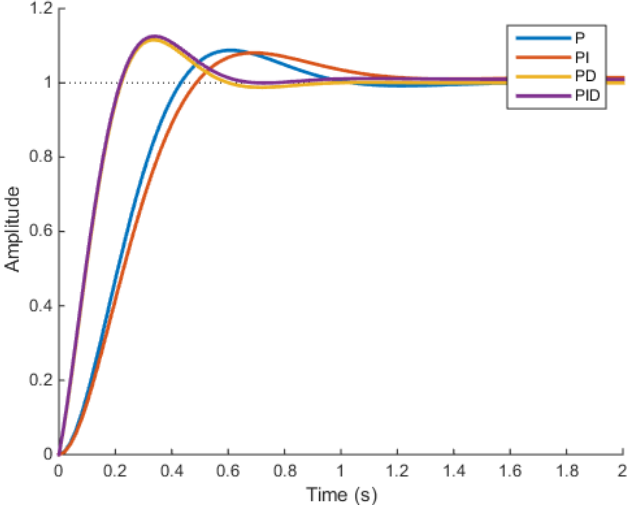
\includegraphics[width = 1 \textwidth]{../img/diagram132.png}
  \caption{Table A-25 | Thermochemical Properties of Selected Substances at 298K and 1 atm}
\end{figure}
\subsection{Evaluating Enthalpy of Ideal Gases}
Enthalpy of any ideal gas $i$ at temperature $T$ (independent of $P$):
\begin{gather}
  \overline{h}_{i}(T) = \overline{h}_{f,i}^\circ + \left[\overline{h}_{i}(T) - \overline{h}_{i}(T_{ref})\right] \\[5pt]
  \text{Absolute enthalpy}  = \text{Enthalpy of formation} + \text{Sensible enthalpy}
\end{gather}
\begin{itemize}[noitemsep]
  \item Enthalpy of formation from its elements (see Table A-25 in text book)
  \item Enthalpy change from reference temperature of 298.15 K
  \begin{enumerate}[noitemsep]
    \item Evaluated from ideal gas Table A-22, A-23 in text book OR
    \item By calculation:
    \begin{gather}
      \Delta \overline{h}_i(T) = \overline{h}_i(T) - \overline{h}_i(T_{ref}) = \int_{298.15K}^{T}\overline{C}_{p}\dif T
    \end{gather}
  \end{enumerate}
\end{itemize}
\section{Closed System Energy Analysis of Combustion}
\subsubsection{Closed Systems:}
In the absence of kinetic and potential energy changes as well as mechanical work, the energy balance equation can be written as:
\begin{align}
  Q + \cancel{W} &= \Delta U_{CM} + \Delta\cancel{KE}_{CM} + \Delta\cancel{PE}_{CM} \\[5pt]
  Q &= U_P - U_R \\[5pt]
  Q &= \sum_{P}n_i\overline{u}_i - \sum_{R}n_i\overline{u}_i \\[5pt]
  Q &= \sum_{P}n_i\left(\overline{h}_i - R_uT\right) - \sum_{R}n_i\left(\overline{h}_i - R_uT\right) \\[5pt]
  Q &= \sum_{P}n_i\left(\overline{h}_{f,i}^\circ + \Delta\overline{h}_{i} - R_uT\right) - \sum_{R}n_i\left(\overline{h}_{f,i}^\circ + \Delta\overline{h}_{i} - R_uT\right)
\end{align}
\section{Heat of Reaction}
\textbf{The heat of reaction (or heat of combustion or chemical heat release)} is the energy released by the oxidation of a fuel under a specified (constant) temperature. \\\\
The heat of reaction is therefore measured by \textbf{keeping the temperature of the reactants and products the same}. It is also dependent on the process (or path) by which it is measured. \\\\
In a constant-volume process, the \textbf{heat of reaction} is the internal energy change, called \textbf{the internal energy of reaction}:
\begin{gather}
  (Q_r)_{T,V} = (\Delta U_r)_{T,V} = U_P - U_R = \sum_{P}n_i\overline{u}_i(T) - \sum_{R}n_i\overline{u}_i(T) \\[5pt]
  = \sum_{P}n_i\left(\overline{h}_{f,i}^\circ + \Delta\overline{h}_{i}(T) - R_uT\right) - \sum_{R}n_i\left(\overline{h}_{f,i}^\circ + \Delta\overline{h}_{i}(T) - R_uT\right)
\end{gather}
In a constant-pressure process, the \textbf{heat of reaction} is the enthalpy change, called \textbf{the enthalpy of reaction}.
\begin{gather}
  (Q_r)_{T,P} = (\Delta H_r)_{T,P} = H_P - H_R = \sum_{P}n_i\overline{h}_i(T) - \sum_{R}n_i\overline{h}_i(T) \\[5pt]
  = \sum_{P}n_i\left(\overline{h}_{f,i}^\circ + \Delta\overline{h}_i(T)\right) - \sum_{R}n_i\left(\overline{h}_{f,i}^\circ + \Delta\overline{h}_i(T)\right)
\end{gather}
\begin{gather*}
  \Delta U_r, \ \Delta H_r < 0 \ \text{for exothermic reaction} \\[5pt]
  \Delta U_r, \ \Delta H_r > 0 \ \text{for endothermic reaction}
\end{gather*}
\subsection{Heat Release of Reaction between Arbitrary Temperatures}
In reality, reactants and products are rarely at the same temperature, not to mention the reference temperature.
\begin{figure}[H]
  \centering
  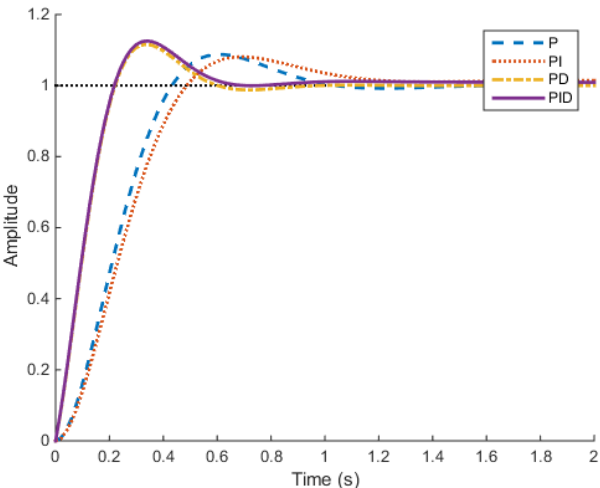
\includegraphics[width = 0.55 \textwidth]{../img/diagram133.png}
  \caption{}
\end{figure}
\subsection{Hess’s Law}
The enthalpy of reaction for a given reaction is the same whether it takes one or several stages to form the same product. \\\\
That is, the enthalpy of reaction is independent of the path of the reaction, but only dependent on the initial and final states. \\\\
For example:
\begin{align}
  (1) &\ C+\frac{1}{2}O_2 \longrightarrow CO + (-110.5 \si{\kilo\joule\per\mole}) \\[5pt]
  (2) &\ CO + \frac{1}{2}O_2 \longrightarrow CO_2 + (-283.0 \si{\kilo\joule\per\mole})
\end{align}
is equilave to:
\begin{gather}
  C + O_2 \longrightarrow CO_2 + (-393.5 \si{\kilo\joule\per\mole})
\end{gather}
\subsection{Heat Release of Reaction between Arbitrary Temperatures}
For a reaction of reactants at $T_1$ and products at $T_2$, the enthalpy of reaction can be determined as follows:
\begin{figure}[H]
  \centering
  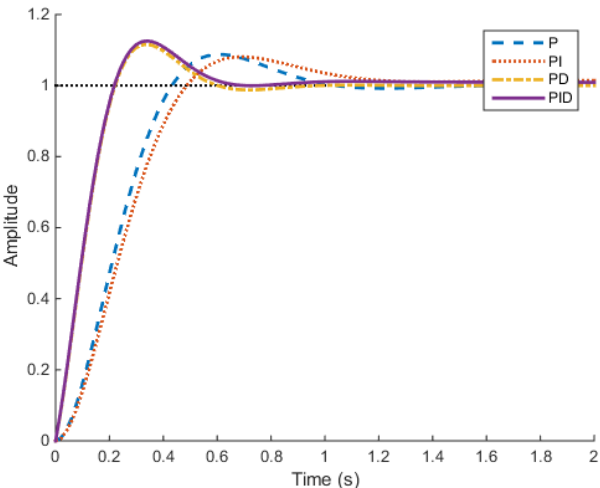
\includegraphics[width = 0.55 \textwidth]{../img/diagram133.png}
  \caption{}
\end{figure}
\begin{gather}
  (Q_r)_{T_1,T_2} = \Delta H_{T_1}^{T_2} = H_P(T_2) - H_R(T_1) \\[5pt]
  = H_P(T_2) - H_P(T_o) + H_P(T_o) - H_R(T_o) + H_R(T_o) - H_R(T_1)
\end{gather}
On a mass basis:
\begin{gather}
  = \sum_{P}\int_{T_o}^{T_2}m_i C_{p,i}\dif T + \Delta H_r^\circ + \sum_{R}\int_{T_1}^{T_o}m_i C_{p,i} \dif T
\end{gather}
On a molar basis:
\begin{gather}
  = \sum_{P}\int_{T_o}^T{T_2}n_i \overline{C}_{p,i} \dif T + \Delta\overline{H}_r^\circ + \sum_{R}\int_{T_1}^{T_o}n_i \overline{C}_{p,i} \dif T 
\end{gather}
The enthalpy of reaction at standard reference conditions:
\begin{gather}
  \Delta H_r^\circ = \sum_{P}m_i h_{f,i}^\circ - \sum_{R}m_i h_{f,i}^\circ \\[5pt]
  \text{OR} \\[5pt]
  \Delta\overline{H}_r^\circ = \sum_{P}n_i\overline{h}_{f,i}^\circ - \sum_{R}n_i\overline{h}_{f,i}^\circ
\end{gather}
\subsection{State of Water in Combustion Products}
\textbf{Water may exist as liquid or vapour in combustion products}, depending on pressure and temperature. \\\\
Relationship between vapour phase and liquid phase enthalpies is given by:
\begin{gather}
  \left(\Delta h_f^\circ\right)_{H_2O,vapour} = \left(\Delta h_f^\circ\right)_{H_2O,liquid} + \left(\Delta h_{fg}\right)_{H_2O} \\[5pt]
  \left(\Delta\overline{h}_f^\circ\right)_{H_2O,vapour} = \left(\Delta\overline{h}_f^\circ\right)_{H_2O,liquid} + \left(\Delta \overline{h}_{fg}\right)_{H_2O}
\end{gather}
Where $\left(\Delta h_{fg}\right)_{H_2O}$ and $\left(\Delta \overline{h}_{fg}\right)_{H_2O}$ are the enthalpy of evaporation in $\si{\joule\per\kilogram}$water and $\si{\joule\per\kilo\mole}$, respectively. \\\\
Note that in text books, $\Delta h_f^\circ$ and $h_f^\circ$ are used interchangeably.
\section{Heating Values of Fuels}
The heating value of a fuel is the magnitude of heat of reaction of a unit composite fuel usually measured in a calorimeter under standard reference conditions (298.15K, 1 atm).
\begin{figure}[H]
  \centering
  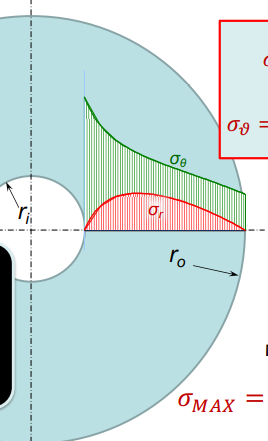
\includegraphics[width = 0.55 \textwidth]{../img/diagram134.png}
  \caption{}
\end{figure}
\begin{enumerate}[noitemsep]
  \item The fuel composition is usually unknown;
  \item The heating value is also called the calorific value;
  \item HHV - higher heating value;
  \item LHV – lower heating value;
  \item $h_{fg,H_2O}$ - enthalpy of evaporation;
  \item For constant volume, $Q_{HV} = |\Delta U_r|$
  \item For constant pressure, $Q_{HV} = |\Delta H_r|$
\end{enumerate}
\begin{gather}
  Q_{HHV} = Q_{LHV} + n_{H_2O}\Delta\overline{h}_{fg,H_2O} \longrightarrow (\si{\joule\per\kilo\mole})\\[5pt]
  Q_{HHV} = Q_{LHV} + m_{H_2O}\Delta h_{fg,H_2O} \longrightarrow (\si{\joule\per\kilogram})
\end{gather}
The values for HHV and LHV for specific substances can be found from Table A-25 | Thermochemical Properties of Selected Substances at 298K and 1 atm.
\section{Adiabatic Flame Temperature}
If all heat evolved during the reaction is used \textbf{solely} for raising the products temperature without heat loss, the final temperature $T_2$ is called the adiabatic flame temperature $T_F$. 
\begin{figure}[H]
  \centering
  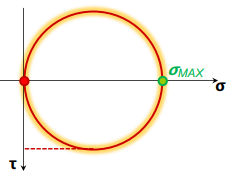
\includegraphics[width = 0.55 \textwidth]{../img/diagram135.png}
  \caption{}
\end{figure}
The adiabatic flame temperature is obtained by setting:
\begin{gather}
  \Delta \overline{H}_{T_1,r}^{T_2} = 0
\end{gather}
And solving the following equation iteratively,
\begin{gather}
  \sum_{P}\int_{T_o}^{T_2}n_i\overline{C}_{p,i}\dif T + \sum_{R}\int_{T_1}^{T_o}n_i\overline{C}_{p,i}\dif T = -\Delta\overline{H}_{r}^\circ
\end{gather}
$T_{F,P}$ is constant-pressure adiabatic flame temperature. \\
$T_{F,V}$ is constant-volume adiabatic flame temperature.
\end{document}